\section{Inputs}

\begin{figure}[H]
    \centering
    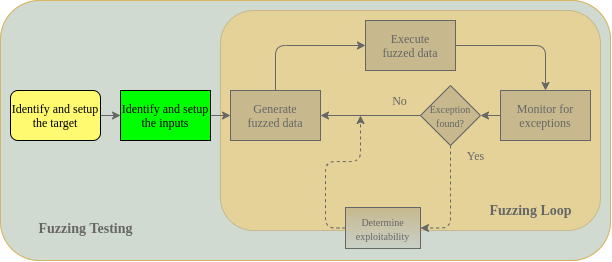
\includegraphics[width=\linewidth]{Chapter3/fuzzing_phase2.png}
\end{figure}

The inputs for our target program are the $x$ values of the functions $f1$ and $f2$. As a result, the input contains two 64-bit float values. 

% To determine the capabilities of Waffle, we parse the input files according to the following format:

% TODO: Define the format here

% The parsed inputs specify the values of the two different variables $x$ and $y$. The domain for each of the variables is $[1]\times[2]$. 